\chapter{Simulation results}

The last step here, is to simulate the power train, related with all the elements inside, as battery bank, power converters, electric motor, etc.

\begin{figure}[h]
    \centering
    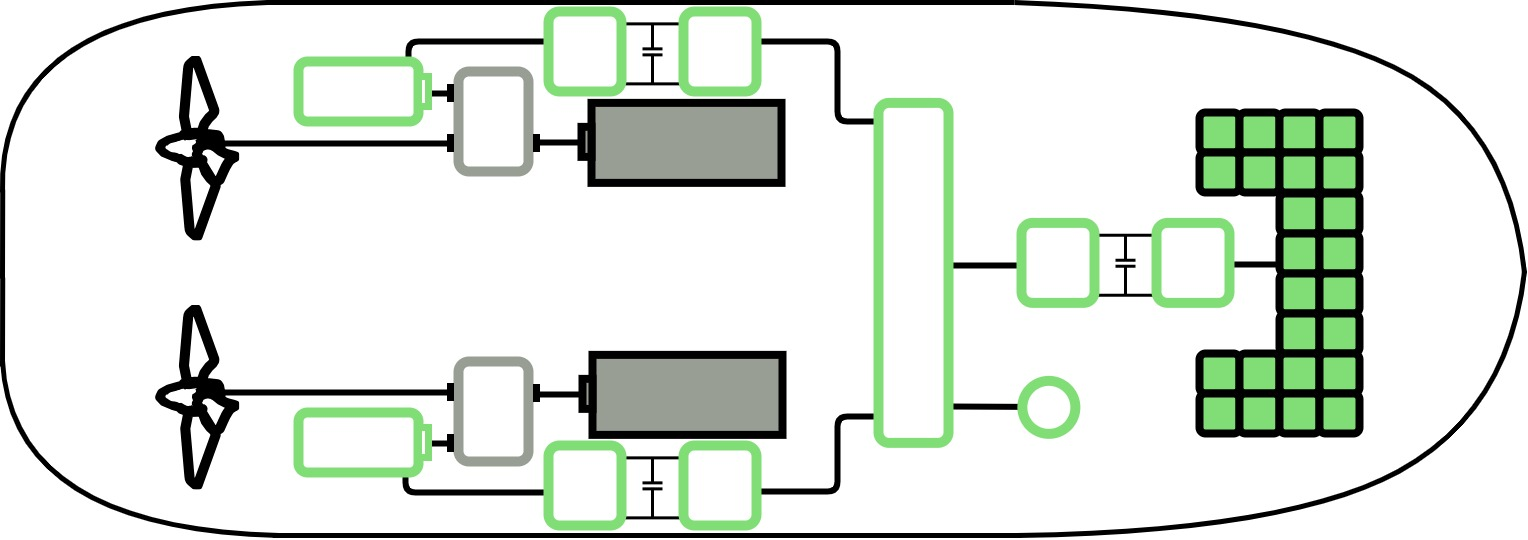
\includegraphics[width=0.75\textwidth]{images/chapter05/PowerTrain.jpg}
    \caption{PowerTrain}
    \label{PowerTrain}
\end{figure}

\section{Battery Cell}

\begin{figure}[h]
    \centering
    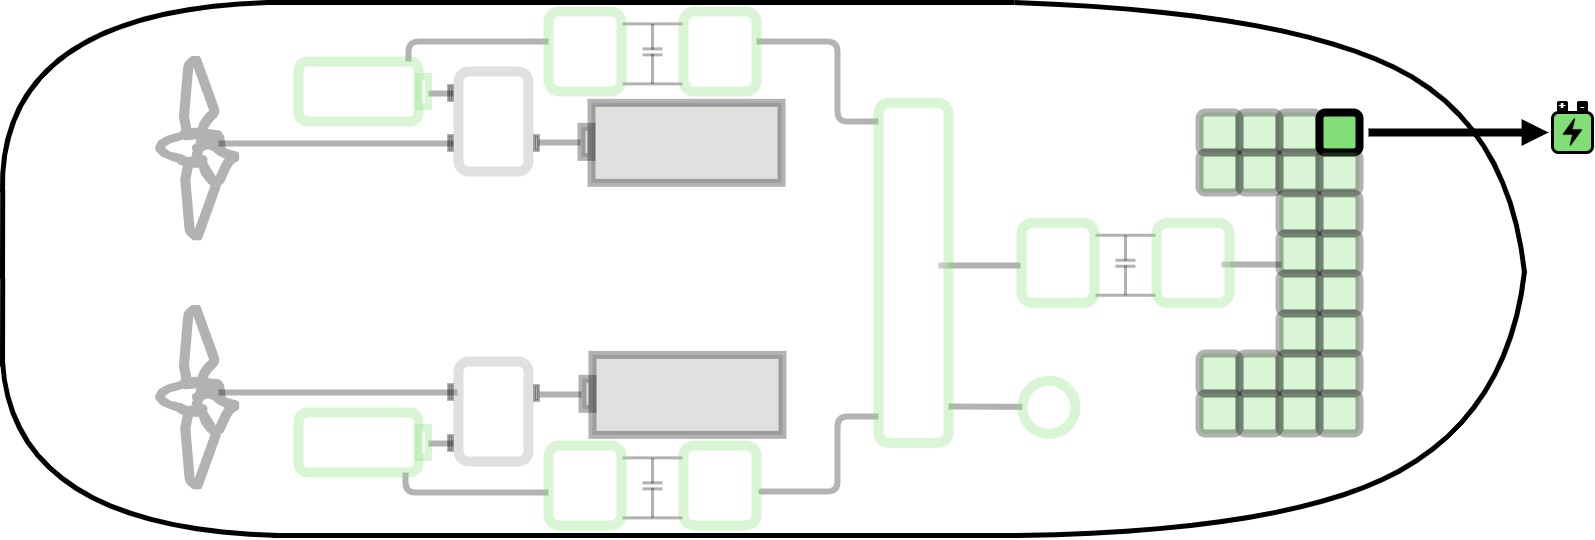
\includegraphics[width=0.75\textwidth]{images/chapter05/01_BattCell/BattCell_scheme.jpg}
    \caption{BattCell in power train.}
    \label{BattCell}
\end{figure}

The battery bank’s design parameters are used to select a cell for electrical modeling with a Shepherd model of order 0. Technical details of the chosen cell, U27-36XP from Valence, are used to find model parameters that closely match its real discharge curve. The model shows good similarity to the actual performance, as illustrated in Fig. 12. This enables the extrapolation of results to model a battery bank and predict its behavior across various operating profiles.

\begin{figure}[h]
    \centering
    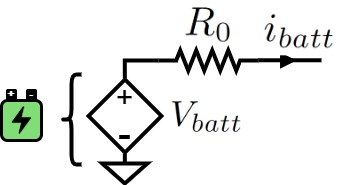
\includegraphics[width=0.3\textwidth]{images/chapter05//01_BattCell/Cell_model.jpg}
    \caption{Cell model zero order Shepherd.}
    \label{fig:Zo_Shepherd}
\end{figure}

\begin{equation}
    V_{batt} = V_0 -K\frac{Q_0}{Q_0-Q}Q + A\cdot e^{-BQ}
\label{eq:Voc}
\end{equation}

\begin{equation}
    Q = \int_0^t i_{batt}(t)dt
\end{equation}

\begin{itemize}
    \item $V_{batt}$: no load voltage [V].
    \item $V_{0}$: Battery constant voltage [V].
    \item $K$: Polarizing voltage/resistance factor [V].
    \item $Q$: Actual battery capacity [Ah].
    \item $Q_{0}$: Battery capacity [Ah].
    \item $A$: Exponential zone voltage amplitude [V].
    \item $B$: Exponential zone time constant inverse [Ah]${}^{-1}$
\end{itemize}

\textcolor{blue}{Agregar imagen de ajuste de curva}

\begin{equation}
\begin{split}
    A &= V_{full}-V_{exp}\\
    B &= \frac{3}{Q_{exp}}\\
    K &= \frac{(V_{full}-V_{nom}+A (e^{-B\cdot Q_{nom}}-1)) \Delta Q}{Q_{full}}\\
   V_0 &= V_{full} + K + R\cdot I_{nom} - A\\
    \Delta Q &=Q_{full}-Q_{nom}
\end{split}
\label{ecuaciones}
\end{equation}



\begin{table}[h]
\centering
\caption{Valores de los parámetros del modelo Sheperd clásico y ajustado para una celda de batería.}
\label{table3}
\begin{tabular}{c|c|c}\hline
Parámetro& Shepherd clásico & Sheperd ajustado\\ \hline \hline 
A& 2.4 [V]& 1.44 [V]\\
B & 3 [$Ah^{-1}$] & 3 [$Ah^{-1}$]\\
K & 1.2857 [V]& 0.0051 [V]\\
$V_0$ & 43.9357 [V]& 39.2536 [V]\\
\hline \hline
\end{tabular}
\end{table}



\begin{figure}[h]

\begin{subfigure}{0.5\textwidth}
    \centering
    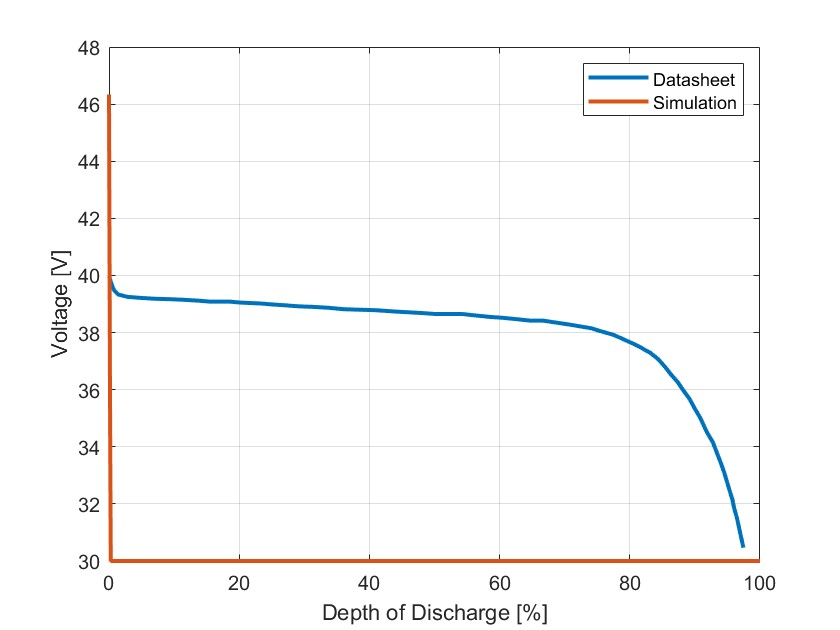
\includegraphics[width=0.75\textwidth]{images/chapter05/01_BattCell/BattCellSim1.jpg} 
    \caption{Classic Shepherd}
    \label{fig:subim1}
\end{subfigure}
\begin{subfigure}{0.5\textwidth}
    \centering
    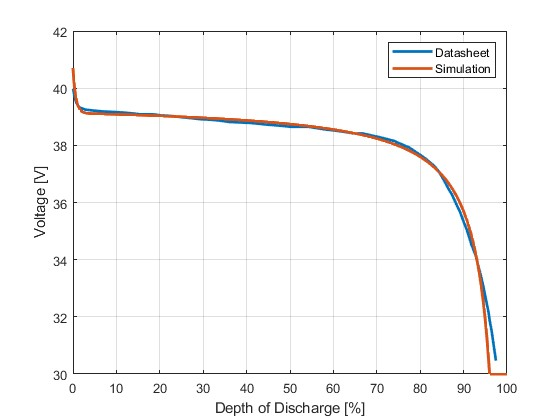
\includegraphics[width=0.75\textwidth]{images/chapter05/01_BattCell/BattCellSim2.jpg} 
    \caption{Adjusted Shepherd}
    \label{fig:subim2}
\end{subfigure}

\caption{Implementation Model of zero order Shepherd.}
\label{fig:image2}
\end{figure}


\section{Battery Bank}

\begin{figure}[h!]
    \centering
    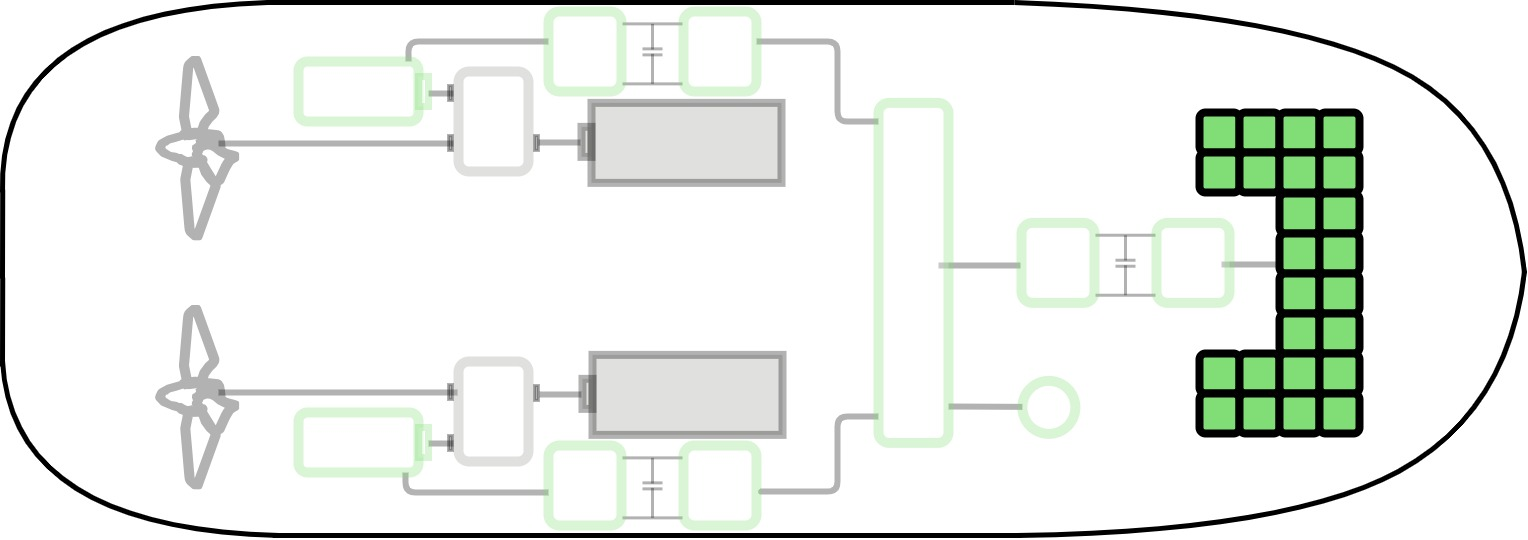
\includegraphics[width=0.75\textwidth]{images/chapter05/02_BattBank/BattBank_scheme.jpg}
    \caption{BattBank in power train.}
    \label{BattBank}
\end{figure}

\begin{table}[h]
\centering
\caption{Valores de los parámetros del modelo Batt Bank}
\label{table4}
\begin{tabular}{c|c}\hline
Parámetro& Shepherd values\\ \hline \hline 
${N}_{s}$ & 19 [-]\\
${N}_{p}$ & 85 [-]\\
A & 27.36 [V]\\
B & 0.0353 [$Ah^{-1}$] \\
K & 0.0011 [V]\\
$V_0$ & 745.7320 [V]\\
\hline \hline
\end{tabular}
\end{table}

\begin{figure}[h!]
    \centering
    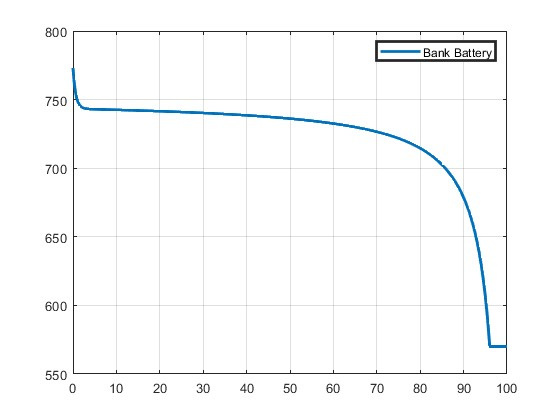
\includegraphics[width=0.75\textwidth]{images/chapter05/02_BattBank/01_VoltageProfile.jpg}
    \caption{BattBank voltage profile.}
    \label{BattBank_vp}
\end{figure}

\begin{figure}[h!]
    \centering
    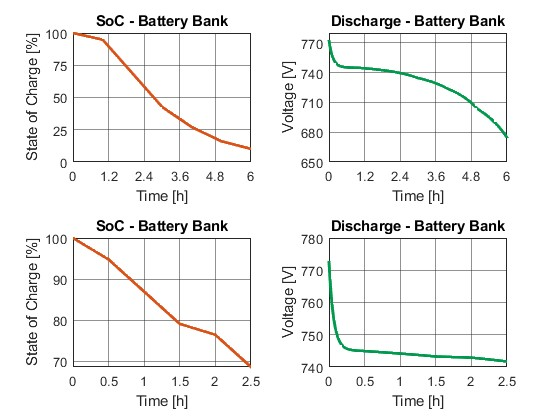
\includegraphics[width=0.75\textwidth]{images/chapter05/02_BattBank/02_ElecBehavior.jpg}
    \caption{BattBank Electrical behavior.}
    \label{BattBank_eb}
\end{figure}

\newpage

\section{Power Converter Battery}

\begin{figure}[h!]
    \centering
    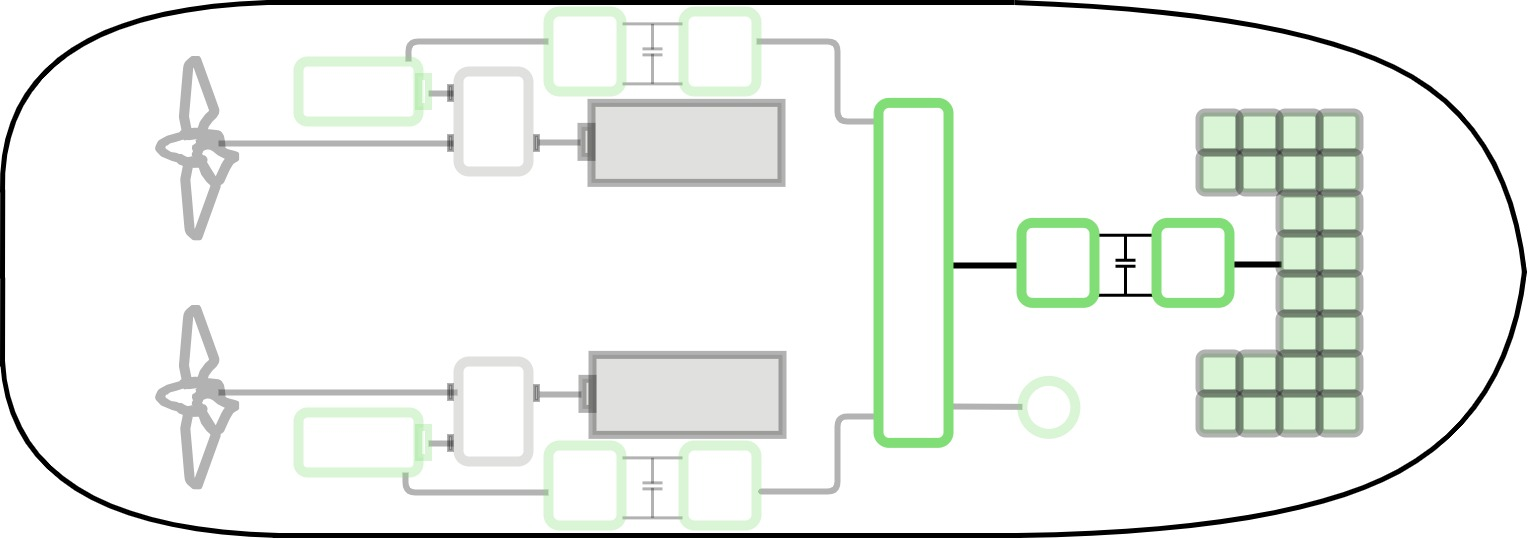
\includegraphics[width=0.75\textwidth]{images/chapter05/03_PowerConverterBatt/PowerConverterBatt.jpg}
    \caption{Power Converter Bank.}
    \label{BattBank_pw}
\end{figure}

\newpage

\section{Electric Motor}

\begin{figure}[h]
    \centering
    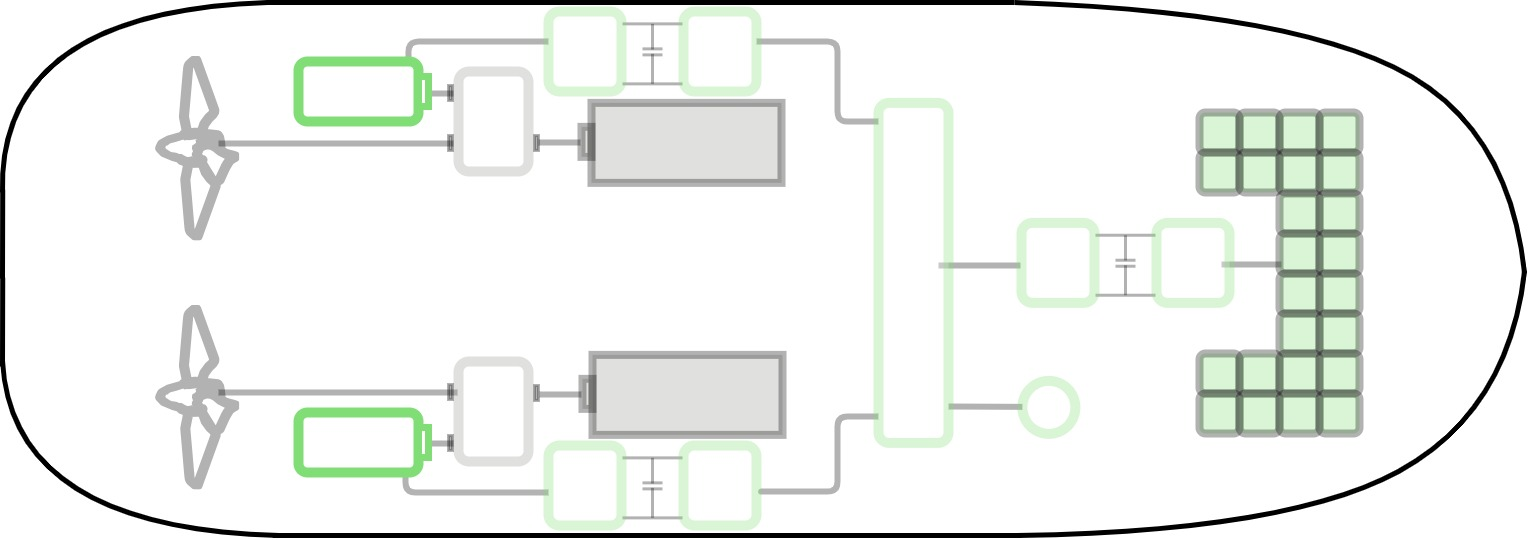
\includegraphics[width=0.75\textwidth]{images/chapter05/ElectricMotor_scheme.jpg}
    \caption{ElectricMotor in power train.}
    \label{ElectricMotor}
\end{figure}

\newpage



\section{Diesel Propulsion Engine}

\begin{figure}[!ht]
    \centering
    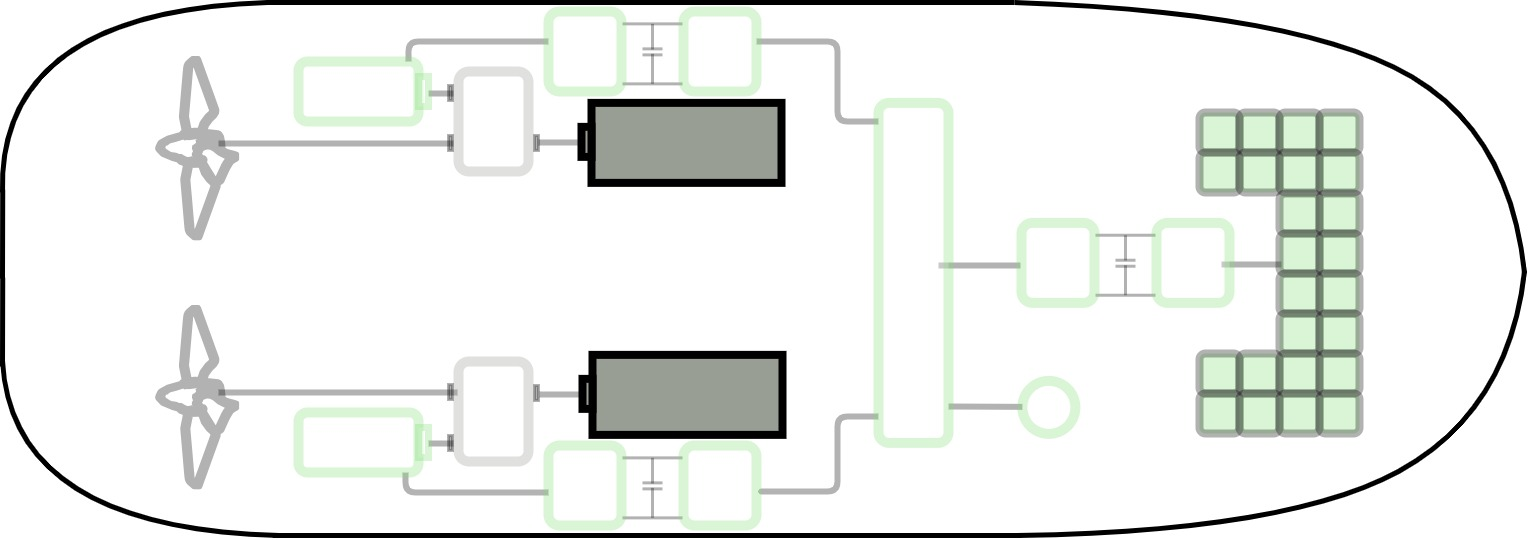
\includegraphics[width=0.75\textwidth]{images/chapter05/DieselEngine_scheme.jpg}
    \caption{Diesel Propulsion Engine in power train.}
    \label{Diesel Engine}
\end{figure}

\section{Propeller}

\begin{figure}[!ht]
    \centering
    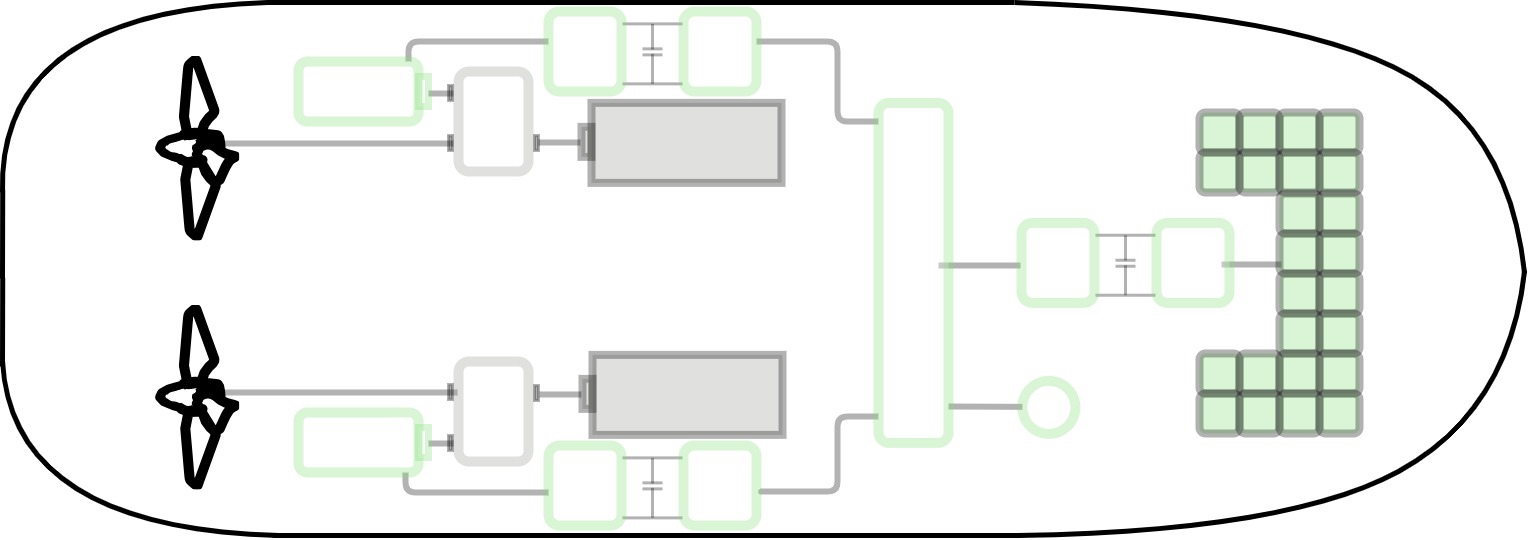
\includegraphics[width=0.75\textwidth]{images/chapter05/Propeller_scheme.jpg}
    \caption{Propeller in power train.}
    \label{Propeller}
\end{figure}

- Explicación
- Curva hélice
- Simulaciones de Potencia